% -*- mode: fundamental -*-

% ****************************************************************

\chapter{RISC-V: the Drum unpipelined CPU}

\markboth{Ch \arabic{chapter}: The Drum CPU code}{\copyrightnotice}

\setcounter{page}{1}
% \renewcommand{\thepage}{\arabic{page}}
\renewcommand{\thepage}{\arabic{chapter}-\arabic{page}}

\label{ch_Drum_code}

% ****************************************************************

\section{Introduction}

In this chapter we use code Drum's behavior, illustrated in
Figure~\ref{Fig_Drum_Instr_Exec}, using BSV's \verb|StmtFSM|
construct.
\begin{figure}[htbp]
  \centerline{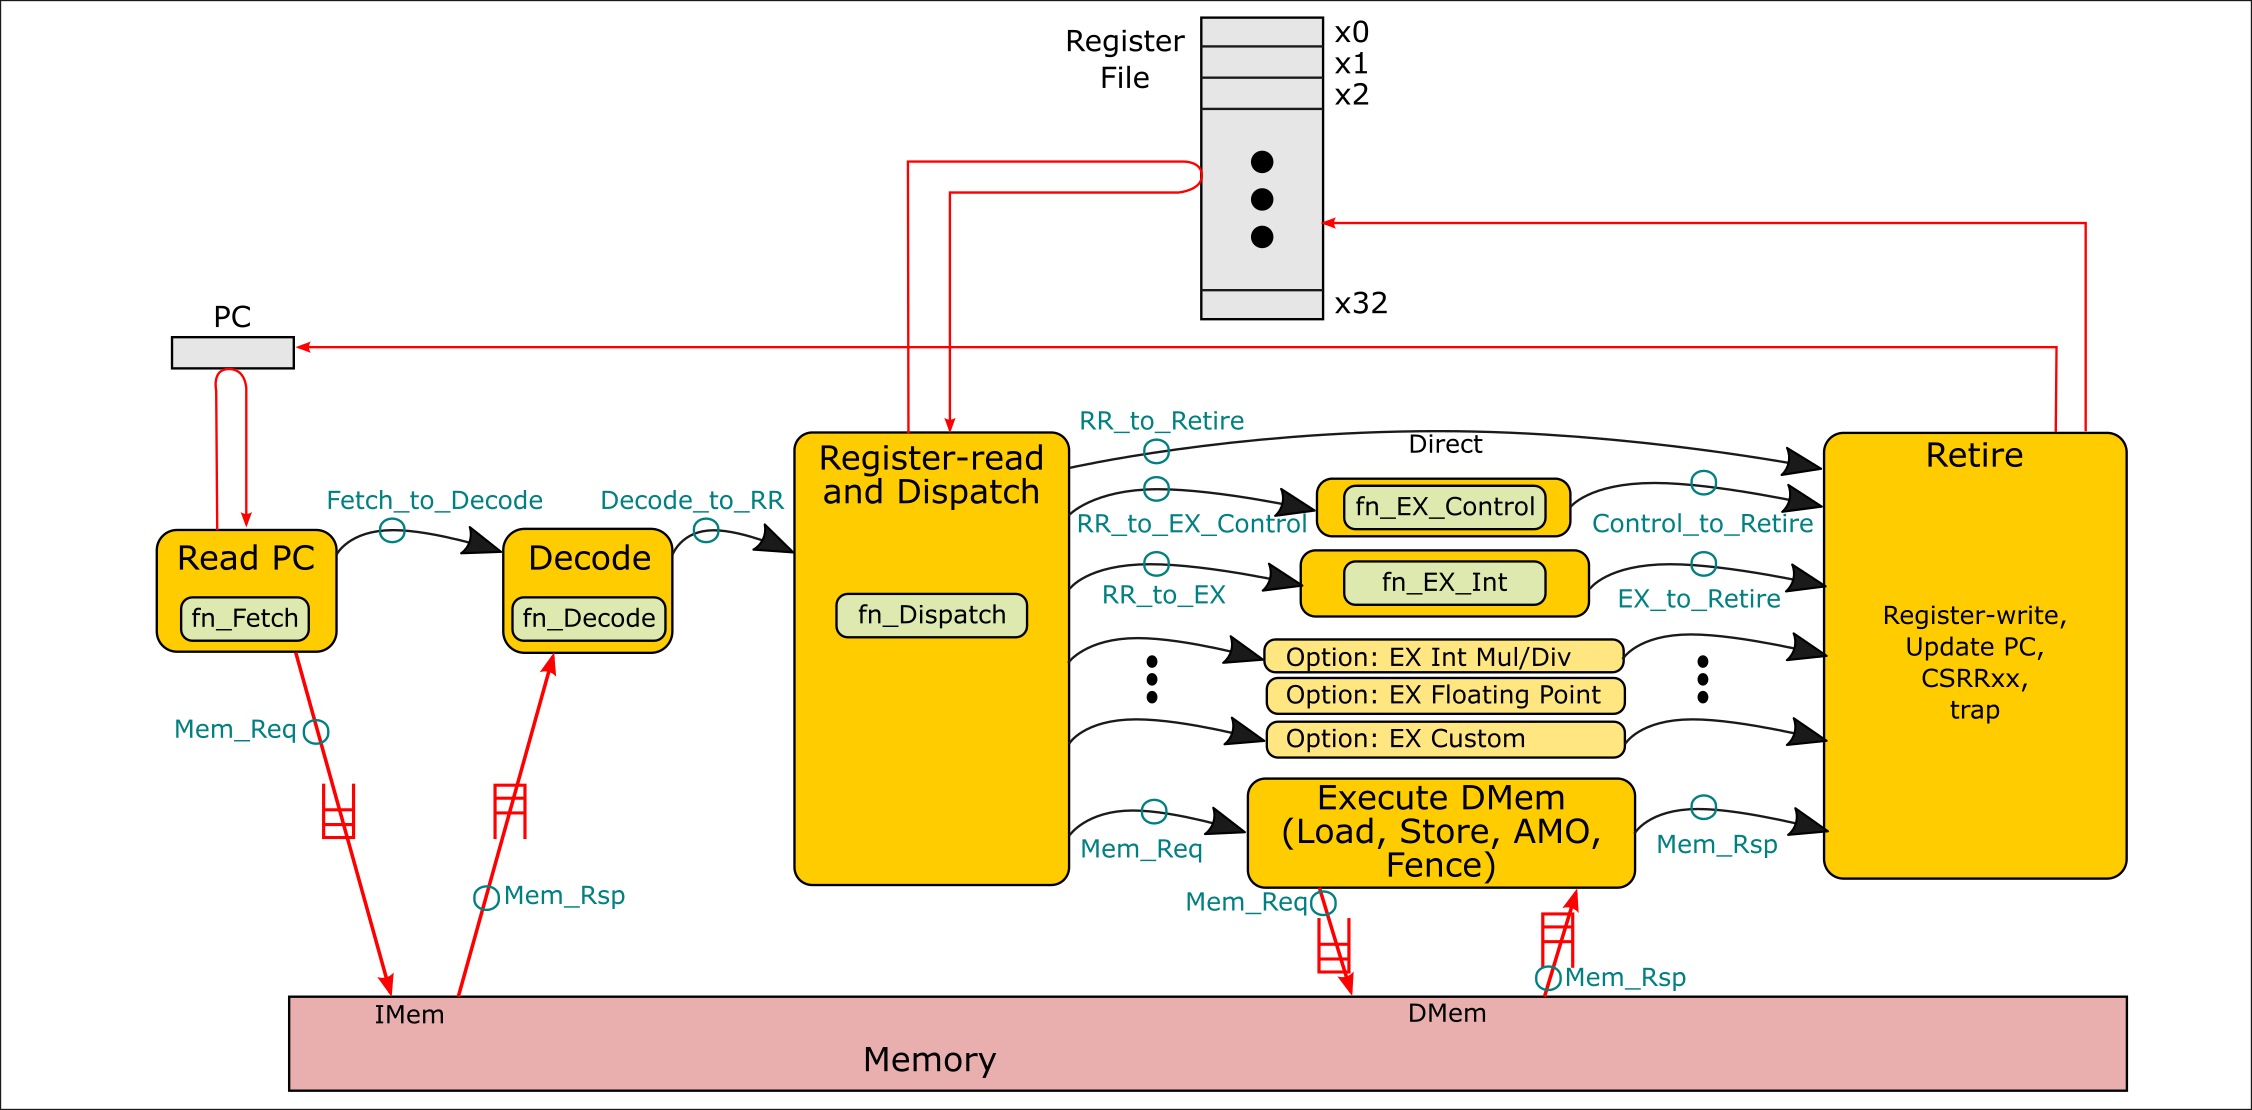
\includegraphics[width=6in,angle=0]{Figures/Fig_Instr_Exec_w_structs}}
  \caption{\label{Fig_Drum_Instr_Exec}
           Simple interpretation of RISC-V instructions
	   (same as Fig.~\ref{Fig_Fetch_function_Simple_Instr_Exec})}
\end{figure}

% ****************************************************************

\section{RISC-V: The interface for the Drum CPU module}

\label{Sec_Drum_CPU_interface}

\index{Drum!CPU interface}

The Drum CPU interface is shown below.

\input{Code_Extracts/CPU_IFC.tex}

The interface is simple:

\begin{tightlist}

  \item The \verb|init| method carries an \verb|Initial_Params| struct
    containing any initial values needed by the CPU.  A typical field
    is the initial value of the PC, since different software systems
    make different assumptions about the ``starting address'' for
    code.  In many RV32I example codes, the starting address is
    \verb|'h_8000_0000|.

  \item A \verb|FIFOF_O| interface to carry memory requests for
    instructions (out-bound from the CPU to the memory);

  \item A \verb|FIFOF_I| interface to carry corresponding memory
    responses containing instructions (in-bound from memory to the
    CPU);

  \item A \verb|FIFO_O| interface to carry memory requests from
    load/store instructions (out-bound from the CPU to the memory);

  \item A \verb|FIFOF_I| interface to carry corresponding load/store
    memory responses (in-bound from memory to the CPU).

\end{tightlist}

(Please re-read Section~\ref{Sec_Harvard_architecture} for the
discussion on Harvard architectures, which have separate memory-access
channels for instructions (Fetch, IMem) and for data (LOAD/STORE,
DMem)).

Later we will see that Fife shares this interface, so that the Fife
and Drum CPUs are easily interchangeable in any system or testbench.

% ****************************************************************

\section{RISC-V: The Drum CPU module}

\label{Sec_Drum_CPU_module}

\index{RISC-V!Drum skeleton module}
\index{RISC-V!Fife skeleton module}
\index{Drum!Skeleton module}
\index{Fife!Skeleton module}

The STATE and INTERFACE sections of the Drum CPU module are shown
below (we will discuss the elided BEHAVIOR section shortly).

\input{Code_Extracts/Drum_mkCPU_STATE.tex}

\hm \emph{(... BEHAVIOR elided, to be discussed shortly ...)}

\input{Code_Extracts/Drum_mkCPU_IFC.tex}

The STATE section first instantiates a register \verb|rg_running|,
initially False, that will be set to True by the \verb|init| method
that initializes the PC to a specific initial value.  The FSM will
wait for this before starting the first instruction-fetch.

Then, \verb|mkCPU| instantiates aa register for the PC, and then the
GPRs module (desribed in Section~\ref{Sec_RISCV_regfile}) and the CSRs
modules (described in Section~\ref{Sec_RISCV_CSRs}).  Then, it
instantiates a set of registers to hold values between temporal FSM
steps (with struct types shown in Figure~\ref{Fig_Drum_Instr_Exec}).
For example, the Fetch step will write a value into
\verb|rg_Fetch_to_Decode| which will be read later by the Decode step.
Then, it instantiates four FIFOFs for IMem requests (outgoing) and
responses (incoming), and for DMem requests (outgoing) and responses
(incoming). As mentioned before, we do not make any assumption about
the \emph{latency} of memory requests, {\ie} how long it takes the
external memory subsystem to consume a request from one of the request
FIFOs and enqueue a response into the corresponding response FIFO.
Finally, it instantiates the four registers needed for trap-handling,
described in Section~\ref{Sec_Traps}.

In this display we have elided the BEHAVIOR section to show just that
we will define the behavior in a \verb|Stmt|, and then use
\verb|mkAutoFSM| (see Section~\ref{Sec_AutoFSM}) to instantiate it
into an FSM and run it.  The first action of the FSM is to wait for
\verb|rg_running| to become true.  We will describe the \verb|Stmt| in
more detail shortly.

In the INTERFACE section, the \verb|init| method initializes the PC
and sets \verb|rg_running| to true, releasing the BEHAVIOR section to
start executing.

In the interface we are using the interface transformers discussed in
Section~\ref{Sec_interface_transfomers} that produce Semi-FIFO
``views'' of FIFOs.

% ================================================================

\subsection{Help-functions for the Drum CPU module behavior}

\label{Sec_Drum_FSM_help_fns}

Before we look at the FSM implementing Drum behavior, we first have
some \verb|Action| functions that encapsulate some common actions
performed in several states in the FSM.

% ----------------
\vspace{2ex}

NOTE:
\fbox{\small
\begin{minipage}{5in}

In BSV, function definitions do not have to be at the top-level of a
file, in fact they can be defined at any nested level.  Here, we
define these inside a module.

\end{minipage}}
% ----------------

The following function writes an rd-value into the the GPRs, in those
cases where the instruction has an rd (\verb|fn_Decode|, described in
Section~\ref{Sec_Decode_Function}, computed \verb|has_rd| for each
kind of instruction):

\input{Code_Extracts/Drum_CPU_upd_rd.tex}

The following function saves values into registers \verb|rg_epc|,
\verb|rg_cause| and \verb|rg_tval|, when a trap is detected.  These
will later be written into the corresponding CSR registers during
trap-handling.

\input{Code_Extracts/Drum_CPU_setup_exc.tex}

This function is the last action during an instruction's execution,
updating the PC and the instruction number:

\input{Code_Extracts/Drum_CPU_redirect.tex}

% ================================================================

\subsection{The Drum CPU module behavior}

\label{Sec_Drum_CPU_module_behavior}

\index{RISC-V!Drum CPU module behavior}
\index{Drum!CPU module behavior}

The Drum CPU module BEHAVIOR for executing a single instruction is
specified using an \verb|FSM|.  This starts with the the Fetch action:

\input{Code_Extracts/Drum_CPU_Fetch.tex}

This applies \verb|fn_Fetch()| (Section~\ref{Sec_fn_Fetch}) to the PC,
stores the \verb|to_D| part of the result in register
\verb|rg_Fetch_to_Decode|, and sends the \verb|mem_req| part of the
result to the Instruction Memory.

The next action in the FSM is the Decode step:

\input{Code_Extracts/Drum_CPU_Decode.tex}

We pop the response from IMem (bind \verb|mem_rsp| to the value at
head of the FIFO, and also remove it from the FIFO), then apply
\verb|fn_Decode()| (Section~\ref{Sec_fn_Decode}) to the
\verb|Fetch_to_Decode| value from the Fetch step and the IMem
response, and store the result in register \verb|rg_Decode_to_RR|.

Recall that each \verb|Action| is instantaneous, and the FSMs sequence
actions.  In the code so far, the Fetch action takes place in one
instant, and the Decode action takes place at a later instant. The
Decode action is not ``enabled'' until an IMem response is available
in the \verb|f_IMem_Rsp| FIFO; it will simply wait until a response is
available.  Thus, the time interval between the Fetch instant and the
Decode instant is unpredictable; it depends on when the IMem result
becomes available (see dicussion in Section~\ref{Sec_mem_latency} on
unpredictable memory latency).

% ----------------
\vspace{2ex}

NOTE:
\fbox{\small
\begin{minipage}{5in}

Looking ahead to a topic we'll discuss in more detail in
Chapter~\ref{ch_Rules}, the FIFO methods ``{\tt .first}'' and ``{\tt
.deq}'', which are used by ``{\tt pop}'' above, have so-called
\emph{implicit conditions}, {\ie} the methods are only ``enabled''
when the FIFO is non-empty.  The Decode action in the FSM is
translated by the \emph{bsc} compiler into a BSV \emph{rule}.  A rule
does not ``fire'' until all the implicit conditions in its
method-calls are enabled.

\end{minipage}}
% ----------------

The next FSM action is the Register-Read and Dispatch step:

\input{Code_Extracts/Drum_CPU_RRD.tex}

Using the information in \verb|rg_Decode_to_RR| created in the Decode
step, we read the two registers \verb|rs1| and \verb|rs2|.  We apply
the function \verb|fn_Dispatch| (Section~\ref{Sec_fn_Dispatch}) and
store the result in register \verb|rg_Dispatch|.

Note that we blindly read both registers \verb|rs1| and \verb|rs2|,
even though many instructions do not have one or both of these fields.
In those situations we'll be reading bogus/irrelevant values, but it
does not matter---in the Execute step we will only use these values in
instructions that need them. Recall that while in a software
programming language this may seem to be unnecessary work, here both
register-read expressions represent real hardware that exists, whether
they are needed for a particular instruction or not.

After the Dispatch FSM step, we move on to the Exectute and Retire FSM
steps.  Figure~\ref{Fig_Retire_Drum} shows the details of the four
``flows'' that may follow.
\begin{figure}[htbp]
  \centerline{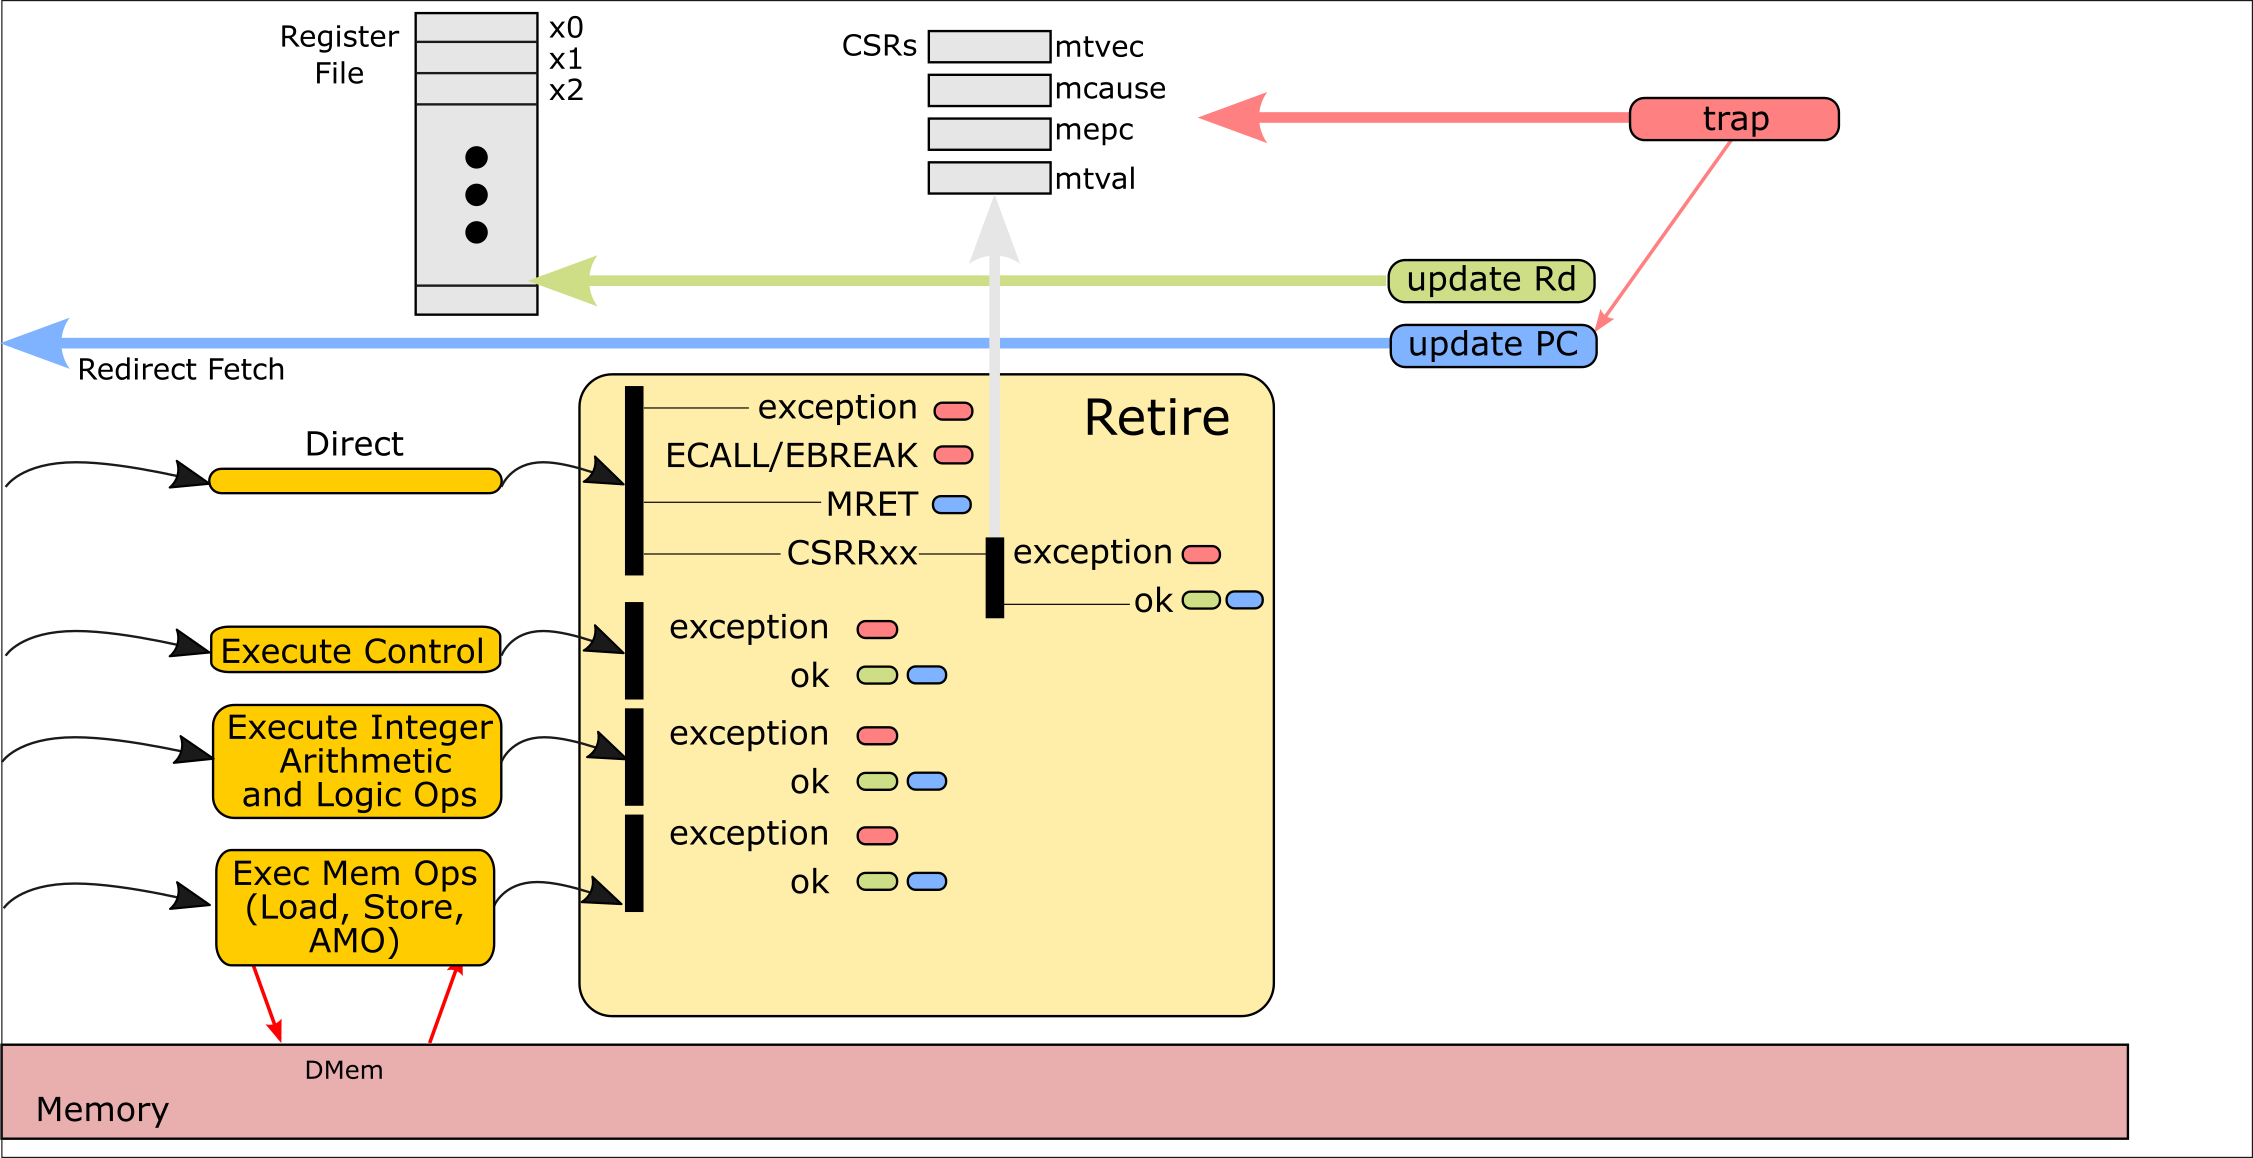
\includegraphics[width=6in,angle=0]{Figures/Fig_Retire_Layers_1}}
  \caption{\label{Fig_Retire_Drum}Execute and Retire actions in Drum}
\end{figure}
Each of the flows can have an exception or a normal (OK) result.  The
Direct flow may need to execute a SYSTEM instruction (ECALL, EBREAK,
MRET and CSRRxx).  Executing a CSRRxx instruction may also have an
exception or normal result.  For each flow, the colored ovals show
what actions may need to be performed; these correspond exactly to the
three help-functions discussed in Section~\ref{Sec_Drum_FSM_help_fns}.

The FSM code follows the structure shown in the diagram.  The
Execute-and-Retire steps of the FSM follow this broad structure:

{\small
\begin{Verbatim}[frame=single, numbers=left, label=Broad sructure of Drum Execute and Retire]
      if (rg_Dispatch.to_Retire.exec_tag == EXEC_TAG_DIRECT)
          ...
      else if (rg_Dispatch.to_Retire.exec_tag == EXEC_TAG_CONTROL)
          ...
      else if (rg_Dispatch.to_Retire.exec_tag == EXEC_TAG_INT)
          ...
      else if (rg_Dispatch.to_Retire.exec_tag == EXEC_TAG_DMEM)
\end{Verbatim}
}

Next we go through each of the four flows (the elided arms in the
above if-then-else).

Direct.

\input{Code_Extracts/Drum_CPU_Direct.tex}

Execute Control

\input{Code_Extracts/Drum_CPU_Control.tex}

Execute Integer

\input{Code_Extracts/Drum_CPU_Int.tex}

Execute DMem

\input{Code_Extracts/Drum_CPU_DMem.tex}

Exceptions

\input{Code_Extracts/Drum_CPU_exc.tex}




Finally, we instantiate a \verb|StmtFSM| module that first waits until
it is allowed to run, and then loops forever, executing one
instruction at a time:

{\small
\begin{Verbatim}[frame=single, numbers=left]
module mkCPU (CPU_IFC);

   ...

   // ================================================================
   // BEHAVIOR

   Stmt exec_one_instr = ...;

   mkAutoFSM (seq
                 await (rg_running);
		 while (True) exec_one_instr;
	      endseq);

   // ================================================================

   ...
endmodule
\end{Verbatim}
}

% ----------------
\hdivider

\Exercise

What might happen if we omitted the ``{\tt await!(rg\_running)}''
statement in the Drum CPU? (Try it in simulation!)

\emph{Hint:} The FSM may start running before the PC has been initialized ...

\Endexercise
% ----------------

% ****************************************************************

\section{RISC-V: Comparing Drum BSV CPU to C code for a RISC-V simulator}

... TO BE WRITTEN ...

% ****************************************************************
